%!TEX root = ../../dissertation.tex
%%%%%%%%%%%%%%%%%%%%%%%%%%%%%%%%%%%%%%%%%%%%%%%%%%%%%%%%%%%%%%%%%%%%%%%%%%%%%%%%
\chapter{Reliable Video Streaming in Mobile Networks}
\label{chap:mobilestreaming}

The analyses of the previous chapter were entirely based on having access to mobile core network measurements. Most research groups will in most likelihood not have this access and have to rely on active end-to-end device measurements or other approaches.

Furthermore, the notion of the importance of reliable video streaming in mobile networks was also not picked up in the previous chapter. Both the load characteristics of mobile networks as well as reliable streaming models were independently investigated up until now. But, as discussed in the beginning of this thesis and suggested in several mobile Internet traffic analyses and forecasts (see for example \cite{cisco2014VNI}), video is already occupying a large portion from mobile traffic and might rise to an even higher ratio in the near future.

Now that the two independent foundations were laid out in the previous chapters, the next two chapters once again merge mobile networks and reliable streaming with two further lines of discussions. 

First, the existing higher layer protocols of a mobile device's reliable video network stack and the influences of lower layer mobile layers on them are analyzed. Contrary to the popular scientific belief, that the Internet is unable to change and renew itself (so called Internet ``ossification'', compare, e.g., \cite{feldmann2010ossification}), protocols in the \gls{TCP}/\gls{IP} stack change all the time. Changes are more likely to occur in the end-to-end stack behavior and not in the packet format, as they are more difficult to change. New application requirements and changing network architectures always trigger adaptations in the stack in-between. Therefore, new and upcoming protocols are presented with an additional focus on the rapid changes to the existing network stack that occurred in the past years.

This also ties in with the mobile network load influencing factors discussed in Section~\ref{c4:sec:loaddefinition}. Any behavior exhibited in the device's stick could also have positive or negative effects on the network's control plane and signaling procedures. The section concludes with a theoretic cross-layer information exchange model that has the potential to improve reliable streaming in scenarios with fluctuating mobile network connections, e.g. during mobility, by informing the streaming application about it and making it possible to react upon such events.

Second, in Chapter~\ref{chap:mobilestreaming-measurements} now that the stack has been discussed fully, several approaches to monitor and measure end-to-end mobile network traffic, and video in particular, are demonstrated and executed. No access to in-network measurement probes limits the level of detail one can deduce from influence sources inside the network. But it also opens up a wide range of other device-based information sources, some of which are crucial in mobile devices, especially regarding mobility. These methods are also not limited to particular mobile network architectures and can thus be used to rapidly compare new architecture evolutions or specific core network implementations to each other. Finally, a full video streaming mobile network simulation model is also presented with some initial results.


%%%%%%%%%%%%%%%%%%%%%%%%%%%%%%%%%%%%%%%%%%%%%%%%%%%%%%%%%%%%%%%%%%%%%%%%%%%%%%%%
%!TEX root = ../../dissertation.tex
%%%%%%%%%%%%%%%%%%%%%%%%%%%%%%%%%%%%%%%%%%%%%%%%%%%%%%%%%%%%%%%%%%%%%%%%%%%%%%%%
\section{Recent Developments in the Mobile Network Stack}
\label{c5:sec:stack-enhancements}


Contrary to the popular scientific belief, that the Internet is unable to change and renew itself (so called Internet ``ossification'', compare, e.g., \cite{feldmann2010ossification}), protocols in the \gls{TCP}/\gls{IP} stack change all the time. Changes are more likely to occur in the end-to-end stack behavior and not in the packet format, as they are more difficult to change. New application requirements and changing network architectures always trigger adaptations in the stack in-between. 

This section briefly covers the existing protocol stacks in relation to mobile networks and streaming, new protocols and how they might influence the stack, and also discusses \gls{TCP} more closely as an example. Beneficial interactions between the stack's layers are presented in a final part.

%%%%%%%%%%%%%%%%%%%%%%%%%%%%%%%%%%%%%%%%%%%%%%%%%%%%%%%%%%%%%%%%%%%%%%%%%%%%%%%%
\subsection{Influences of the Existing Stack}

Superficially not much has changed in the Web's protocol stack. There is still \gls{IP}, \gls{TCP}, and \gls{HTTP} forming effectively the same protocol stack since 1991 with HTTP/0.9. And this seems hard to change, especially the transport layer is fixed to \gls{UDP} and \gls{TCP}, everything else will probably get rejected, altered or even dropped by one of the numerous middleboxes, such as \glspl{NAT}, or forced ``traffic optimization'' transparent proxies, all of which are especially prevalent in mobile networks \cite{sigcomm11middleboxes}. As a side note, this adds another layer of state kept in the network. A fact that was already discussed as being highly problematic and capable of inducing load in the core network in Chapter~\ref{chap:mobilenets}.

Each protocol, representing a layer in the stack, characteristically contributes to influencing data transmissions and varies in its degree of impact on the network as well as the intended goal of the transmission (e.g., streaming and watching a video).

\begin{figure}[htb]
	\centering
	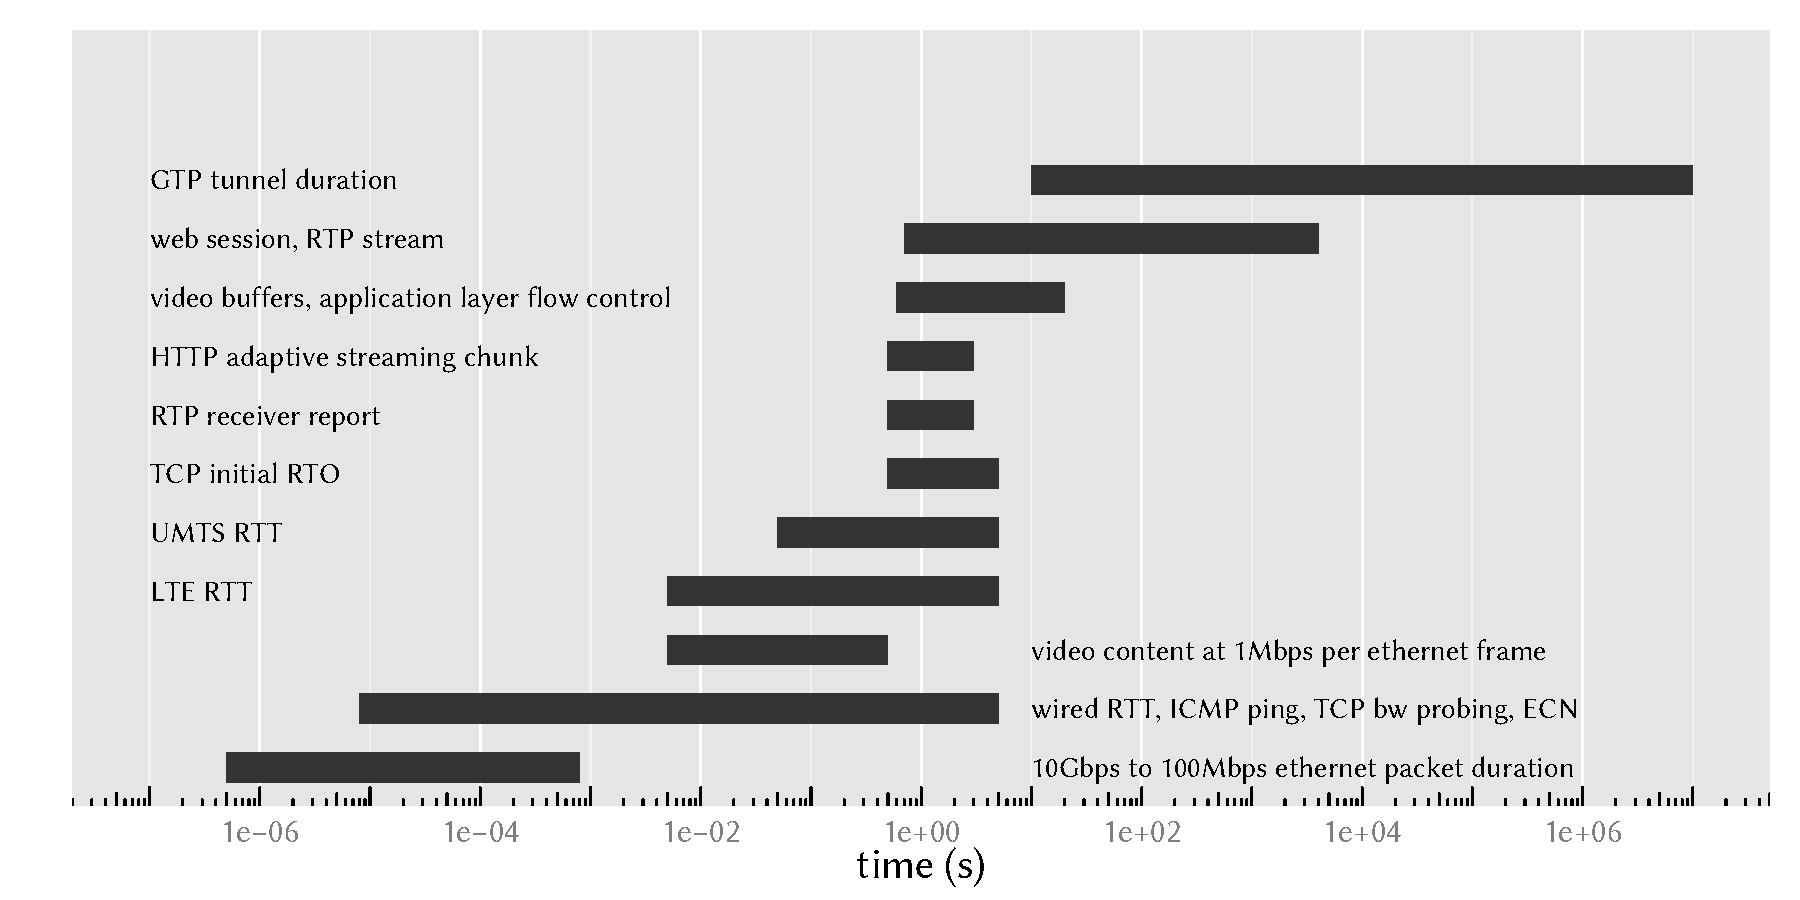
\includegraphics[width=1.0\textwidth]{images/layer-timescales.pdf}
	\caption{Approximate discernible time scales the networking stack protocols operate on in each layer.}
\label{c5:fig:timescales}
\end{figure}

Associated with each layer, and with the actual application running on top of the stack as well, are different timing constraints or time constants of control. Figure~\ref{c5:fig:timescales} overviews the approximate time scales on which activities take place, spanning a remarkable range of twelve orders of magnitude. Complexity is introduced by stacking multiple layers on top of each another, with many layers bringing along their own notion of control and feedback loops. Functionality might be duplicated across different layers, e.g., flow control in the application and on transport layer, leading to nested control loops, which might be coupled due to the timing constraints.

From the application layer end-to-end perspective the mobile network protocols seem to simply increase the depths of the protocol stack. Still, there are effects present that are specific to wireless access and mobile networks differ from the notion of an underlying wired ``dumb'' bit pipe.

First, typical effects of wireless connectivity relating to physical phenomena like fading and interference can be observed. Interruptions in the radio link are a major source of packet loss and spiking delay.
The overall delay in a mobile network is also strongly dependent on the mobile network technology used and has considerably decreased over the last few specification evolutions, even the core network. This was investigated in  \cite{laner2011dissecting3gdelay}. But even with the latest version is the \gls{RAB} and \gls{gtp} tunnel setup --- as previously described in \ref{c4:3gpparchitecture} --- sufficiently lengthy to be measurable and influence packet delay on initiating connections \cite{arlos2010packetsizedelayinfluence}.

To save radio and network resources devices usually have to quickly release their alloted slots causing additional delay for applications during connection reestablishment. Moreover, mobile networks offer many control options and parameters that can further influence any of the upper layers. Mobile devices have the tendency to be somewhat sensitive to some of these changes. For example, the authors of \cite{sigcomm11middleboxes} show the impact from protocol manipulations conducted by middleboxes. 

Comparing all these factors to wired protocols such as 802.3 Ethernet it is clear, that much more can happen in the mobile stack. Today Ethernet is a point to point protocol, transmission delay depends only on very few predictable factors, such as the distance. Wired access is typically not conducted solely through Ethernet, but with access technologies such as \gls{DSL} using \gls{PPPoE} or cable with \gls{DOCSIS}. While they also add more layers to wired access, they should be by far less influencing than the mobile stack. The latter has to additionally manage mobility and the shared wireless radio medium with protocols such as \gls{RLC} and \gls{RRC}.

A further details is the interaction between mobile network frame sizes and the \gls{IP} \gls{MTU}. Usually \gls{IP} adapts its packet size to the shortest frame size of all the link layer links in the path using \gls{PMTU} discovery as described in \cite{rfc1191}. Unfortunately, this can not work in \gls{3G} mobile networks, user packets are transparently fragmented by the radio protocols to fit into the transmission slots alloted to the device. For example, a \gls{GPRS} transmission slot has a length of only \SI{576.9}{\micro\second} carrying just \SI{114}{\bit}. And in \gls{UMTS} \SI{40}{\byte} of payload are typically carried in each \gls{RLC} frame (with optional header compression in the \gls{PDCP} layer).

% http://etutorials.org/Mobile+devices/gprs+mobile+internet/Chapter+1+Introduction+to+the+GSM+System/Radio+Interface/
% http://books.google.at/books?id=Vk9AmYz7TfoC&pg=PA184&lpg=PA184&dq=umts+pdu+size&source=bl&ots=jeO-rpM8HK&sig=NB2FAB37YcdyujYUt_kaHYwLEOE&hl=en&sa=X&ei=KjCxU6C-FKip0AXh94GQDw&redir_esc=y#v=onepage&q=umts%20pdu%20size&f=false

This fragmentation is another source of an undesired interaction between \gls{3G}'s link layer and everything above and including the network layer, potentially fragmenting packets over a long period and thereby causing delay.

In a neutral network, all packets are treated the same and should be subject to the same \gls{RTT} influencing sources.
However, delays in the delivery of data to the upper layers can occur due to certain protocol features, such as \gls{TCP} retransmissions. After being detected through timers or duplicate acknowledgments any lost packet is automatically retransmitted by the sender. Therefore, loss from the lower layers is hidden from the application layer at the cost of delay variations and probably increased overall delay. The increase in delay is especially noteworthy in any \gls{3G} cellular network with its notion of link layer \gls{ARQ} and mobility. With the latter concept, transmissions originally running through one radio tower are redirected to a new tower after a handover, even if the handover period was lengthy. These two combined can be the source of very high delay, reaching seconds to even hundreds of seconds, when moving quickly between coverage areas (e.g., in a car or train). 
This also causes bad interactions with \gls{TCP}, as these long-delayed segments are thought to be lost and subsequently retransmitted, resulting in an even further increase of delay and delay jitter.


% ! <-- !

Another undesirable side-effect of middleboxes, but also of any other network node on the path are overdimensioned packet buffers and the bufferbloat effect caused by them.

%%
Bufferbloat, Congestion Control, and AQM Effects on Reliable Mobile Streaming

 ECN~\cite{rfc3168} (one of the earlier notions of cross-layer interactions; disabled by default almost everywhere)

Comparison of end-to-end and network-supported fast startup congestion control schemes \cite{scharf2011comparison}

Bufferbloat: Dark Buffers in the Internet \cite{gettys2011bufferbloat}

Detecting and quantifying bufferbloat in network paths \cite{groenewegen2011detecting}

Congestion avoidance and control \cite{jacobson1988congestion}

Controlling Queue Delay \cite{Nichols:2012:CQD:2209249.2209264} CoDel\cite{nichols2014codel}
 TCP needs congestion loss to determine bottleneck line speed
	too much buffering hinders this
 Memory is cheap, so why not put in some more megabytes
 Home router buffer induced latency can be as high as several seconds
CoDel:
 Head drop not tail drop
 Queues only as shock absorbers
 What matters is the delay within a flow
 CoDel measures minimal packet pass through time in the local device buffer during a defined interval
 If minimum gets too high, too much buffering is happening
 If delay value does not once fall below a target in the interval CoDel will start dropping packets
	Signals congestion and hopefully reduces source rate
	If stays above target, progressively more packets are dropped
	Target: 5ms; interval: 100ms, based on simulation results
 Can be enabled in Linux since 3.5, but many NIC drivers do not support it yet
 Every buffer along the path influences transmission
	Most impact on the node before the bottleneck
	Cell towers, dsl/cable modems, ...

%Application Layer Protocols

using TLS or not

Firefox Patch: Sort Idle HTTP Connections by CWND \cite{ffSortCWND}

There exists a diversity of streaming applications and associated application-layer protocols, each supporting to differing degrees certain types of streaming, and each having its own set of requirements:
\begin{itemize}
\item Content type --- Pre-generated (as for example in case of video sharing web sites) or live (e.g. televised sports events, news feeds)
\item Codec --- adaptive, variable, or constant media bitrate
\item Playback control and quality feedback --- client/server-side, implicit/explicit
\end{itemize}
Adhering to the design space limits present on the Internet, most innovation takes place on the application layer.
With each streaming protocol come slightly different time scales and feedback loops. Looking at reliable streaming...


%Application Behavior
As indicated in Figure~\ref{c5:fig:timescales}, the time scale on which streaming applications buffer content lie in the range of seconds. This is a necessity in a best-effort network, as the available network bitrate might drop unexpectedly and could drain a shallower buffer quickly. On the other hand, given sufficient bandwidth, buffer sizes could be reduced, improving interactivity of the stream and enabling closer-to-realtime live streaming or conferencing.
Buffering and playback strategies in current applications are such a pivotal point in the operation of video streaming in mobile networks as discussion in Chapter~\ref{chap:streaming}.

%Cross-Layer Influences
Layered network models often assume the functional separation of network layers. The timescales shown in Figure~\ref{c5:fig:timescales} partly support this notion, but also show that there are conflicts in the speed of control loops that can be implemented. Indeed, actual protocols and hardware need to be aware of and often explicitly exploit cross-layer influences and information flow.
\gls{TCP} is an example for this: Its tracking of a congestion window reflects not the state of the transport, but of the network and lower layers. Congestion is assumed by \gls{TCP} if segments are lost (or unduly delayed) below the transport layer. Consequently, if loss happens on the lower layers for reasons other than congestion, \gls{TCP} reacts in an inappropriate way. As indicated in the previous section, loss and delay spikes may have many root causes in a wireless network, and loss might be concealed altogether through lower-layer retransmission methods.
Another example concerning \gls{TCP} is the \gls{PMTU} discovery. Here, \gls{TCP} probes the largest segment size that can be transmitted by the host-to-network layer in one transmission, e.g., Ethernet frame, using \gls{IP}'s ``Don't Fragment'' signaling. Again, a mobile network does not behave the same way an \gls{IP}/Ethernet-based network would work, as it conceals its actual \gls{MTU} and reports it can transport full Ethernet frames.
In addition to (probably inadvertent) behavioral differences between ``classical'' wireline / Ethernet-based and cellular mobile Internet, an \gls{LTE} mobile network typically lies within the administrative domain of one single operator, and thus offers significantly more control over data flows. Through appropriate policies tailored to the user, their subscription model, and other factors such as the overall network status, bearers in the network can be configured for all types of services. Depending on the bearers' quality settings, the operator can support (or, to the contrary, penalize) streaming traffic.

The problem of protocols drawing wrong conclusions due to wireline assumptions has been described for \gls{TCP} above. It is foreseeable that a similar set of problems will appear when operators enforce different policies on Internet-based services without checking first the applicability of their traffic engineering methods. The methodology presented in this deliverable will help to understand beforehand the effects on the user that bearer quality settings have. Similarly, the methodology will present a set of tools to judge before engineering new hardware the capability of certain controls envisioned by the standards bodies, and if an implementation would turn out useful for a set of streaming services.
%%% end insert










%%%%%%%%%%%%%%%%%%%%%%%%%%%%%%%%%%%%%%%%%%%%%%%%%%%%%%%%%%%%%%%%%%%%%%%%%%%%%%%%
\subsection{Upcoming Protocols and Streaming Relationship}

Improvements to congestion control for mobile streaming?


 Alternative modes of transport (e.g. DCCP, , RED, Google's SPDY or new approaches)

 Alternate Transport Protocols (DCCP\cite{rfc4340}, LEDBAT\cite{rfc6817}/$\mu$TP\cite{bt2010utp}, QUIC, SCTP~\cite{rfc4960}, DTLS~\cite{rfc6347})

but successful protocols develop de-facto; de jure much harder (see \gls{3G})



 End-to-end encryption and Authentication mechanisms (e.g.IPSec~\cite{rfc4301}, DNSSEC~\cite{rfc4033}, \gls{DANE}~\cite{rfc6698})


\gls{QUIC}  Quick UDP Internet Connections; protocols without retransmission feature (lost packets are not relevant and cause head-of-line blocking) but still with the all-important congestion control + TLS
%http://www.ietf.org/proceedings/88/slides/slides-88-tsvarea-10.pdf
\footnote{\url{http://lwn.net/Articles/558826/}}
UDP based for now, could very well end up as modifications to future TCP
inherits new TCP features such as TFO, snap start, ...
avoids most retransmissions through FEC
congestion control not through CWND but through packet pacing
includes stream multiplexing and TLS-like crypto by default



WebSocket \cite{rfc6455}
WebSockets as streaming transport \cite{w3c2011websockets} \cite{heise2011websockets}
 IETF HyBi (Hypertext Bidirectional) Working group
 W3C WebSocket API
 Supported by every major browser and Web server
 Provides full-duplex client-server communication
	Upgrades from HTTP/1.1 through extension header
	Barebone protocol atop TCP (or TLS), not HTTP
	HTTP/1.1 only allows client-initiated polling (GET)
	Asynchronous server push possible
		In HTTP/1.1 only achievable through various hacks (e.g. ``long polling'')
		Stateful instead of stateless (as HTTP)
Lower overhead per transmission/frame
Reduces number of open TCP connections and bandwidth overhead (no polling on additional TCP connection)


WebRTC \cite{webrtcdraft}


SPDY: An experimental protocol for a faster web \cite{google2011SPDYdef} and \cite{google2010SPDYwp} 
SPDY / \gls{HTTP}/2.0 (multiplexing -> segmented streaming)
 Google proposal and draft
	Currently SPDY/3.1 
	IETF httpbis working group basis for http/2.0
 original Draft based on Chrome browser implementation
 Widespread use and implementations
	Chrome, Firefox; Apache, Nginx
	Google, Twitter, Facebook, Akamai, Wordpress, ...
	HTTP-requests are transparently upgraded through Next Protocol Negotiation
 TLS mandatory
 HTTP/1.1 syntax still viable as a layer on top of SPDY
 Aim: Just one connection held per domain
	Better server scaling (less concurrent connections, fewer packets sent)
	Better latency
Multiplexing/Streams:
 Control and Data Frames, with header compression
 Stream interleaving/multiplexing or cancellation
 Server hint
	Server informs client, what he might want to request in the near future
 Server created streams / server push
	Avoiding one additional RTT and polling
	Only data pushed related to possible GET requests
	Client-side throttles to prevent ``push attacks''
 Stream priorities (8 levels)
	Prefer essential resources over others (images)
	Prefer data with earlier deadlines? (E.g. load next few video streams immediately while already requesting more)
 Use with Scalable Video Coding (Base Layer vs Enhancement Layers)?
 Per stream flow control
multiplexing:
 HTTP: One file request after another
	Pipelining usually absent or disabled by default in browsers (Chrome, Firefox, IE)
	High complexity/maintenance, low gain, head-of-line blocking issues
 SPDY: File parts reordered according to timelines
	Out of order and interleaved requests
Evaluations:
	Average reduction in page load time: ~29\%; 27\% - 60\%
	Strongly dependent on connection, server environment
	HTTP/1.1 optimization (resources split on multiple domains) prevents SPDY multiplexing gains
 SPDY could be more susceptible to packet loss and TCP congestion window downscaling
	Only one connection used compared to multiple HTTP/1.1
 Possible operator benefits
	Significant reduction in concurrent TCP sessions
	Reduction in packets per second
	$\rightarrow$ Reduced infrastructure load?
spdy mobile page load times
 Chrome on Android tests with several Websites
 Emulated mobile conditions (constant 2Mbps, 150ms RTT)
 ~23\% average load time reduction
 Benefits can be higher for large RTT
	Less request round trips and connection setups needed



HTTP/2.0~\cite{http20draft}
 HTTP/1.0 defined in 1996, 1.1 in 1999
	Since then no changes changes to the core protocol
 Many long standing issues with HTTP/1.1, e.g.
	Problems with ``long fat pipes''
		Many parallel connections as workaround
		Fairness issues
	Large overhead for small requests
 IETF Hypertext Transfer Protocol Bis Working Group
 Initial call for proposals made in March 2012
 Planned 2.0 standard proposal in 2014/2015
 Using SPDY as a starting point
 General aims
	Tackle multiplexing, improve load times and experienced latency
	But preserve the semantics of HTTP/1.1
requires presence (but not usage) of TLS1.2
	if used, emphemeral cipher suites >=2048 must be used (a.k.a. Perfect Forward Secrecy)












%%%%%%%%%%%%%%%%%%%%%%%%%%%%%%%%%%%%%%%%%%%%%%%%%%%%%%%%%%%%%%%%%%%%%%%%%%%%%%%%
\subsection{The TCP Case: Prime Example of a Living, Ever-Evolving Protocol}

\gls{TCP} changes (Fast Open, IW10, ...; any relationship to streaming? maybe faster)

SACK or no SACK, CUBIC, ...

% most data from kernelnewbies.org
\begin{table}[htb]
	\begin{tabu}{X[1.4]XX[0.4]X[0.7]}
	\toprule
	\textbf{Change} & \textbf{Related Standard} & \textbf{Kernel} & \textbf{Date} \\
	\midrule
	BIC as default congestion avoidance algorithm (from Reno) & & 2.6.8 & August 2004 \\
	CUBIC as default congestion avoidance algorithm & \cite{ha2008cubic} & 2.6.19 & November 2006 \\
	New TCP Slow Start: HyStart & \cite{Ha20112092} & 2.6.29 & March 2009 \\
	Multipath TCP & RFC6824 & external & 2011 \\
	TCP User Timeout & RFC5482~\cite{rfc5482} & 2.6.37 & January 2011 \\
	Initial Receive Window \SI{10}{MSS} & \cite{rfc6928} & 2.6.38 & March 2011 \\
	Initial Congestion Window \SI{10}{MSS} & RFC6928~\cite{rfc6928} & 2.6.39 & May 2011 \\
	\SI{1}{\second} initial RTO (from \SI{3}{\second}) & RFC6298 & 3.1 & October 2011 \\
	Changes to sstresh and CWND bevahior & RFC5681~\cite{rfc5681} & 3.1 & October 2011 \\ % details: https://git.kernel.org/cgit/linux/kernel/git/torvalds/linux.git/commit/?id=9ad7c049f0f79c418e293b1b68cf10d68f54fcdb
	TCP Proportional Rate Reduction & RFC6937~\cite{rfc6937} & 3.2 & January 2012 \\
	Byte queue limits and TCP buffer limits &  & 3.3 & March 2012 \\ % https://lwn.net/Articles/454390/
	CoDel AQM & \cite{nichols2014codel} & 3.5 & July 2012 \\
	TCP Early Retransmit & RFC5827~\cite{rfc5827} & 3.5 & July 2012 \\
	TCP small queues & & 3.6 & September 2012 \\ %http://lwn.net/Articles/507065/
	TCP Fast Open (client side) & \cite{cheng2014tcptfo} & 3.6 & September 2012 \\
	TCP Fast Open (server side) & & 3.7 & December 2012 \\
	TCP tail loss probe & & 3.10 & June 2013 \\ % http://tools.ietf.org/html/draft-dukkipati-tcpm-tcp-loss-probe-01
	TCP Forward RTO-Recovery & RFC5682~\cite{rfc5682} & 3.10 & June 2013 \\
	Low latency network polling & & 3.11 & September 2013 \\ %http://lwn.net/Articles/551284/ and http://www.linuxplumbersconf.org/2012/wp-content/uploads/2012/09/2012-lpc-Low-Latency-Sockets-slides-brandeburg.pdf
	Improved RTO calculation and handling of reordering & & 3.12 & November 2013 \\ % https://git.kernel.org/cgit/linux/kernel/git/torvalds/linux.git/commit/?id=0f7cc9a3c2bd89b15720dbf358e9b9e62af27126 and https://git.kernel.org/cgit/linux/kernel/git/torvalds/linux.git/commit/?id=ed08495c31bb991de636d2488abaa50b39f2ff4a
	TCP Fast Open enabled by default & & 3.13 & January 2014 \\
	TCP auto corking & & 3.14 & March 2014 \\ % https://git.kernel.org/cgit/linux/kernel/git/torvalds/linux.git/commit/?id=f54b311142a92ea2e42598e347b84e1655caf8e3
	PIE AQM & & 3.14 & March 2014 \\ % http://tools.ietf.org/html/draft-pan-aqm-pie-01 and https://git.kernel.org/cgit/linux/kernel/git/torvalds/linux.git/commit/?id=d4b36210c2e6ecef0ce52fb6c18c51144f5c2d88
	TCP Fast Open over IPv6 & & 3.16 & 2014 \\
	\bottomrule
	\end{tabu}
	\caption{Assorted list of some select network stack changes in the Linux kernel, that alter \gls{TCP}'s transmission bevahior.}
\label{c5:tab:linux-stack-changes}
\end{table}

Also look at ``An in-depth study of LTE: effect of network protocol and application behavior on performance'' \cite{Huang:2013:ISL:2486001.2486006}

TCP modifications for short-lived connections (e.g. initially ignore congestion avoidance and push a lot of data at once (google.com approach, Increasing TCP's Initial Window)) 

IW10: better response time, still fair \cite{rfc6928}
An argument for increasing \gls{TCP}'s initial congestion window \cite{dukkipati2010argument}
IW3, IW10  Initial window size (IW10, ...)
 TCP Congestion Window
	Maximal number of packets in flight
–	Scaling through congestion control and avoidance algorithms
 Initial Value
	1 (RFC1122, RFC2001)
	4000 Bytes (~ 3 packets) (RFC2414, RFC3390, ~2002)
	IETF proposal: IW10 (Google Draft 2010-2012)
 Rationale
	HTTP request for small websites using new TCP connection
	Transmit whole site in one RTT instead of multiple
	Reduces average latency
		Evaluation: ~10\% page load reduction on typical web pages
	High IW values already used by many CDNs



TCP Fast Open~\cite{cheng2014tcptfo}
 IETF draft
 Linux 3.6 client side implementation (September 2012)
 Linux 3.7 server side (~ 2012)
 Small server-side application adaptation required
 Send data in the SYN and SYNACK packets
	Deliver it immediately to the application
	Only allowed for subsequent connections, requires additional security cookie (specific to client-server IP pair)
 Saves one initial RTT
 4\% to 41\% popular web page load time improvement


1s / 3s Retransmission Timeout \cite{rfc6298}
 TCP retransmission timeout set through RTT measurement
 Default value needed for timeouts during handshake: 3 seconds (now obsolete RFC1122, RFC2988)
 RFC 6298, Linux 3.1 (October 2011)
	Reduce TCP initial retransmission timeout to 1 second
 Improves TCP handshake times for lossy networks
 Benefits for short-lived (Web) transactions


Proportional Rate Reduction PRR (RFC 6937 \cite{rfc6937} vs. rfc 3517)
 TCP behavior on packet loss in the past
	RFC 3517: reduce CWND to half
		Must first ACK large portion of the data still in flight before transmitting again
	Linux: ``Rate halving''; Reduce CWND by 1 on every ACK until CWND/2
		Can still send data during recovery
 Google IETF Proposal (Linux 3.2, January 2012): PRR
	Reduce timeouts by avoiding excessive window reductions
	Converge to cwnd chosen by congestion control by the end of recovery
	Can improve packet loss recovery time and average latency



TCP Early Retransmit \cite{rfc5827} Kernel 3.5 (July 2012)
 TCP loss recovery (not using SACK) triggers on
	Timeout (may be lengthy, ~RTT, min 1s)
	Triple duplicate ACK (fast retransmit)
		If CWND is small, TCP may not be able to get enough DUPACKs to trigger
		Reduce DUPACK threshold for these connections
 Reduce DUPACK threshold for these connections
	Less robust to segment reordering
 Reduces average latency for narrow and lossy connections

Multipath TCP MPTCP~\cite{rfc6824}!


Congestion Avoidance algorithm ((New Reno~\cite{rfc6582}, Vegas~\cite{Brakmo:1994:TVN:190809.190317}, Compound~\cite{song2006compound}, BIC, CUBIC~\cite{ha2008cubic}; all w or w/o SACK)
general basic tcp congestion control in \cite{rfc5681}, describing Reno

Slow Start~\cite{rfc5681}
 HyStart~\cite{Ha20112092}


Nagle's Algorithm~\cite{rfc896} delaying and aggregating small data packets


OS-dependent receive window scaling behavior

OS-dependent choice of packet size


%%%%%%%%%%%%%%%%%%%%%%%%%%%%%%%%%%%%%%%%%%%%%%%%%%%%%%%%%%%%%%%%%%%%%%%%%%%%%%%%
\subsection{Proposal for Cross-Layer Enhancements}
\label{c5:crosslayerhinting}


Wired Internet access has a very narrow choice of protocols on the \gls{ISO}/\gls{OSI} Layers 1 and 2. The typical use-case consists of a \gls{LAN} using Ethernet which is then tunneled through or translated into one of several access technologies, e.g., \gls{DSL}, \gls{DOCSIS}, or \gls{PON}. Applications often make assumptions that rely on the presence of these protocols and their specific characteristics.

However, Internet access today is similarly often achieved using mobile cellular networks. The latest standardized iteration of these is \gls{LTE} and the accompanying \gls{EPS} core network infrastructure \cite{olsson2009sae}. This is the first evolution of standards that completely removes the classical circuit switched domain making room for more radio frequency bandwidth to be used with the all-\gls{IP} services achieving shared transmission capacities --- comparable to today's 802.11n WiFi --- albeit on much larger cell sizes of \SI{1}{\kilo\meter} to \SI{3}{\kilo\meter}. The \gls{EPS} network acts as an intermediary between the radio access stations and the Internet enabling strong traffic control mechanisms as well as mobility anchored at the \gls{SGW}. Traffic is routed through the core by using tunneling over the \gls{SGW} and \gls{PGW} based on the traffic bearer concept defined either in the \gls{gtp} or the \gls{PMIPv6} protocols. For every mobile device connected to the network there is one default and up to ten dedicated bearers carrying traffic filtered by pre-set \gls{QoS} parameters. Control is enforced through a logically separate network control plane, that is also used to setup and tear down these bearers. Figure fig:ltestack displays the disparity between the Internet's protocol stack and that of an \gls{LTE} network encapsulating all user traffic in additional protocol layers by the tunneling process.

Research work is ongoing how to best work with this complex network setup. It is expected, that with the rise of mobile access the core network comes under heavy traffic pressure with negative affects on the \gls{QoS} of best-effort traffic. Endeavors are required to study the loaded network's behavior. Also very little work has gone into exploring the control plane characteristics of these networks, including their performance. A novel approach could also be, to make mobile device applications, e.g. video streaming players, aware of the core networks capabilities and allow the request of tunnels tailored to their specific \gls{QoS} requirements resulting in a possible increase of perceived quality.

% influence of signaling plane and core network elements - scaling

The protocols used for the radio transmissions behave very differently when compared to Ethernet and assumptions made by higher layers may not hold any more. This can apply to, e.g., reliability, frame sizing and fragmenting, and latency amounting to undesired effects on higher-layer traffic. For example, loss in \gls{GSM} and \gls{UMTS} networks is often caught transparently on layer 2 and a retransmission is conducted. However, in the time the retransmission takes the transport layer may have already run into a timeout and re-requested the missing segment on its own, resulting in additional delay and a waste of bandwidth. This is especially detrimental for time-critical applications like video streaming, possibly resulting in buffer underruns and degraded quality. Transport and application layer mechanisms need to be able to understand this and cope with the effects. E.g., \gls{TCP} retransmissions and congestion control could be adjusted in the course of understanding this.

Furthermore, traffic could be avoided during cell handover occurrences. This would require cross-layer cooperation and an awareness of the application when an handover is supposed to occur. The application then could schedule its traffic accordingly. Traffic falling into a handover is subject to especially high latency and loss because the mobile network acts as a mobility anchor which needs to internally reroute incoming traffic to the mobile device's new position. \gls{HTTP} traffic is especially suited to this scheduling behavior because of its statelessness and consistence of small objects that can be requested and transferred independently.


\subsubsection{Related Work}

\begin{itemize}
	\item Cross-layer design optimizations in wireless protocol stacks \cite{Raisinghani2004720}
	\item ECLAIR: An efficient cross layer architecture for wireless protocol stacks \cite{raisinghani2004eclair}
	\item Still no implementation of ECLAIR: ``Cross-layer feedback architecture for mobile device protocol stacks'' \cite{1580937}
	\item 802.21
	\item A multi-layer mobility management architecture using cross-layer signalling interactions\cite{wang2003multi}
	\item 
		\begin{itemize}
			\item \gls{DLEP} \cite{ietf2013dlepdraft}
			\item running on routers for communication between routers and attached interfaces (wireless!)
			\item interface/modem informs router about link characteristics
			\item router acts upon this information
			\item specific set of required and optional signals (message types / reason for messaging) and data items (information)
			\item bandwidth, latency, connection status (loss)
			\item information about specific neighbors
			\item \gls{UDP}-based, discovery mechanism via multicast, session-based
			\item requires/relies on lower layer auth/crypt
			\item no data items specific for cell-type mobile nets and mobility
			\item best suited for routers with external modems/interfaces (outside antennas)
		\end{itemize}
	\item Seamless Mobility in Heterogeneous Wireless Networks \cite{zarai2010seamless}
	\item Radio resource management in emerging heterogeneous wireless networks \cite{Piamrat20111066}
	\item Improved community network node design using a DLEP based radio-to-router interface \cite{6379143}
	\item Cross-layer signalling for next-generation wireless systems \cite{1200522}
	\item Cross-layer design for wireless networks \cite{1235598}
	\item A cautionary perspective on cross-layer design \cite{1404568}
	\item User-centric mobility management for multimedia content access \cite{bolla2011usercentric}
	\item Socketless \gls{TCP} --- an end to end handover solution \cite{1635680}
	\item SATSIX cross-layer architecture \cite{4656786}
	\item mostly routing protocol optimization oriented ``A cross layer based QoS model for wireless and mobile ad hoc networks'' \cite{krishna2007cross}
	\item SmoothIT mechanisms; lower layer elements provide information to higher layers, overlays\footnote{\url{http://www.smoothit.org}}  \cite{oechsner2009pushing}
	\item ``Mobility Awareness'' \cite{hummel2010mobilitaet} PMLAR (Predictive mobility and location-aware routing protocol in mobile ad hoc networks)
	\item Automatic Multi-interface Management Through Profile Handling \cite{Bonnin:2009:AMM:1503496.1503498}
	\item A ubiquitous mobile communication architecture for next-generation heterogeneous wireless systems \cite{1452832} (supposed to propose a function that determines the best handover initiation time in order to avoid early or late initiations)
	\item Optimized video streaming over 802.11 by cross-layer signaling \cite{1580941}
	\item LCP Link Control Protocol, PPP extension RFCs \cite{rfc1570,rfc1661}
 	\item Modem Link Properties Advertisement Protocol\footnote{\url{https://tools.ietf.org/html/draft-ivancic-mobopts-modemlpa-01}}
	\item IEEE 802.21 cooperative handovers, but with required network support
	\item LISP and other mobility approaches \cite{rfc6830}
	\item Radio Resource Management RRM
		\begin{itemize}
			\item resource monitoring, decision making, decision enforcement
			\item choose available wireless interfaces  best suited for a specific task
			\item rudimentary implementations in mobile OSs
		\end{itemize}
\end{itemize}




%%
\subsubsection{Cross-Layer Mobility Hinting}

Today's mobile networks are all of a cellular design. A device that moves from one cell to the other has to perform a so-called handover. During this process the device is deregistered in one cell and registered in the new one. All network traffic currently in flight has to be rerouted or relayed to the device's new location. 
Although seemingly transparent to the device's application, adverse side effects can occur during a handover, including an increase and variability of latency. 

Mobility support today always means network assisted mobility. Typically, the network decides the best possible mobility strategy from its point of view and provides infrastructure to support seamless handovers in the form of mobility anchor nodes. However, the device is actually in a very unique position, as it knows a great deal more about its traffic mix, its currently running applications and its user than the network ever could and should.
Unfortunately, most of this information remains unused, as today's network infrastructures and lower layer protocol stacks provide only very slim changes to exert control over decisions regarding the device.

Nonetheless, a lot could still be done when providing the device's operating system and application ecosystem with a simple bidirectional pathway for vertical information and control flow across network protocol layers and to other low-level systems. This work aims to do just that by providing a generic interface and exchange protocol for any kind of information relevant to an application's decision making process. With this meaningful actions and reactions of individual layers can be defined and tested. Possible use cases are provided in the next section.

Still, one has also to keep in mind, that layering and encapsulation is there for a reason and violating this is a rather risky undertaking. However, we do not think that our approach actually violates these basic principles and only extends on the ways one can communicate and interact with all individual layers without changing anything in them.


	% - Research objectives
	% 	- Bidirectional vertical information and control flow on the performance of the individual layers
	% 		- Definition of generic interfaces
	% 		- Definition of a protocol (including information types, etc.)
	% 	- Definition of meaningful actions/reactions on the individual layers (e.g. adaptation of real-time communication data sources or changes in resource allocation)

		

\subsubsection{Scenario Use Cases}

\begin{itemize}
	\item Video/Voice calls that notify the other party, that interruptions are expected to occur.

	\item Using current location data and movement patterns/predictions to improve cell selections and initiate horizontal and vertical handovers to a time suitable for the device and running applications.

	\begin{figure}[htb]
	        \centering
	        \begin{subfigure}[b]{0.90\textwidth}
	            \centering
				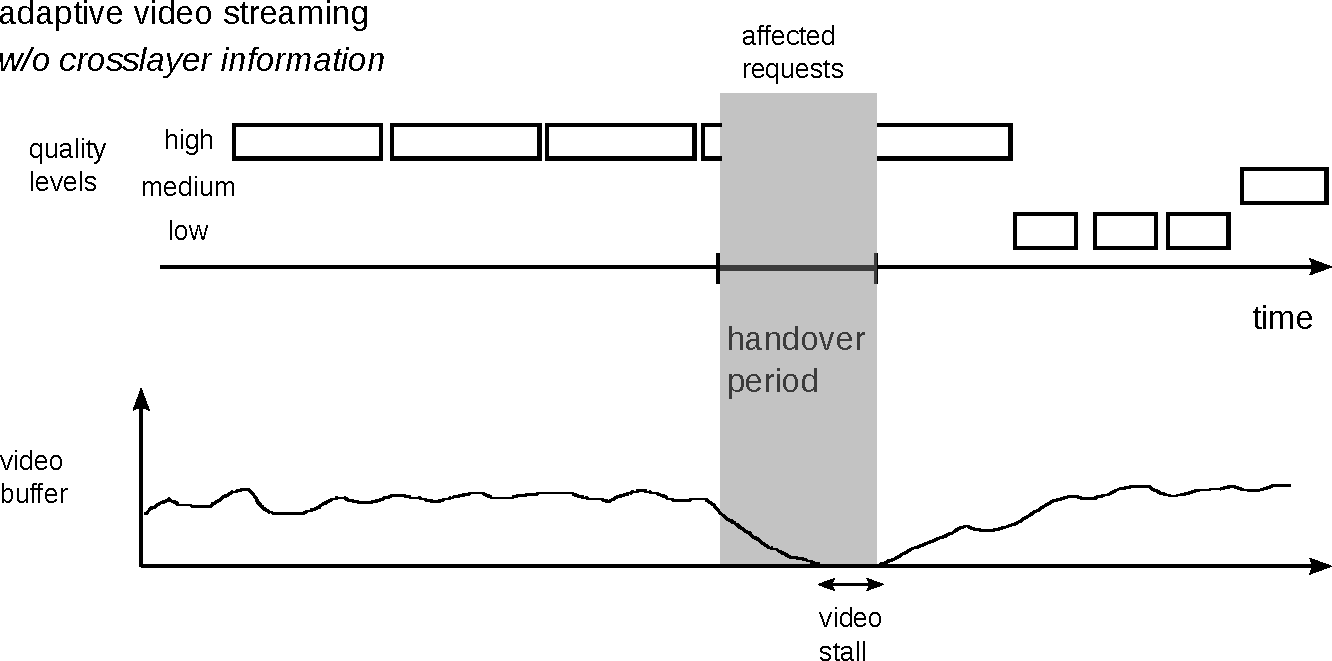
\includegraphics[width=\textwidth]{images/adaptive-streaming-no-cl.pdf}
				\caption{Stalling occurs without handover hinting.}
				\label{c5:fig:streaming-hinting-no-cl}
	        \end{subfigure}%

	        \begin{subfigure}[b]{0.90\textwidth}
				\centering
				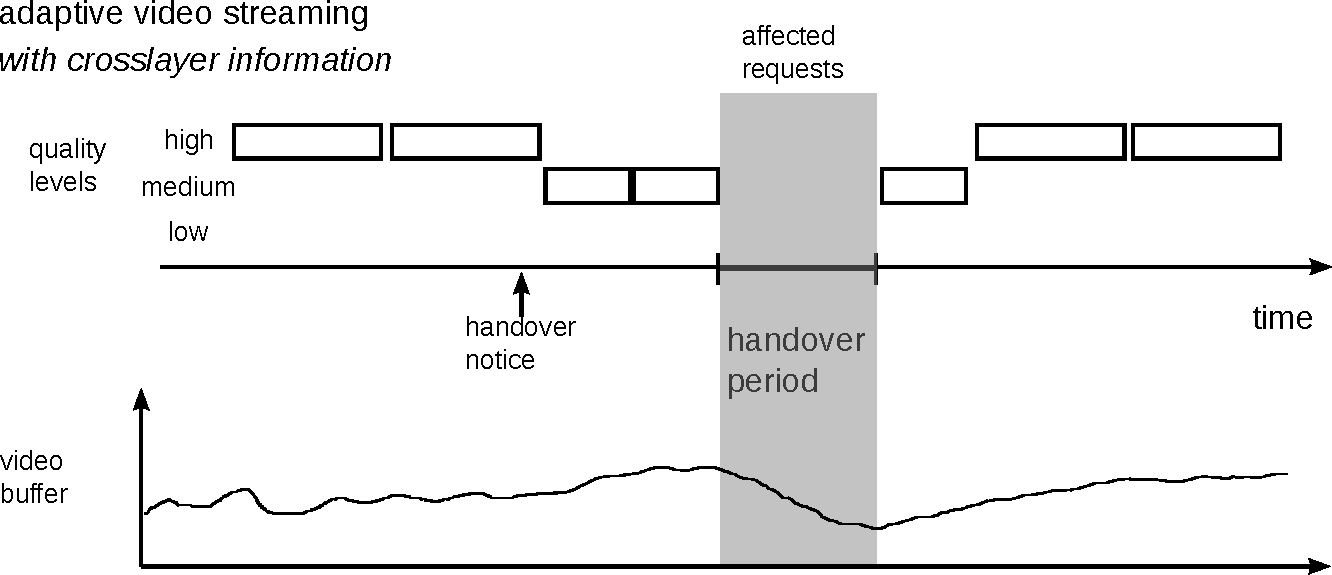
\includegraphics[width=\textwidth]{images/adaptive-streaming-cl.pdf}
				\caption{Stalling can be prevented by hinting and proactively filling the playback buffer.}
				\label{c5:fig:streaming-hinting-cl}
			   \end{subfigure}%
	 \caption{Mockup of handover prediction and hinting for adaptive streaming and thus avoiding playback stalls.}
	\label{c5:fig:streaming-hinting}
	\end{figure}

	\item An adaptive streaming video application increases its video buffer when a shortly upcoming handover is announced to survive the service outage. This can be achieved by an increased rate of segment retrieval and a reduction in segment quality. The goal is to avoid any possible playback stalls due to the handover. Figure~\ref{c5:fig:streaming-hinting} demonstrates this circumstance.

	\begin{figure}[htb]
	        \centering
	        \begin{subfigure}[b]{0.90\textwidth}
	            \centering
				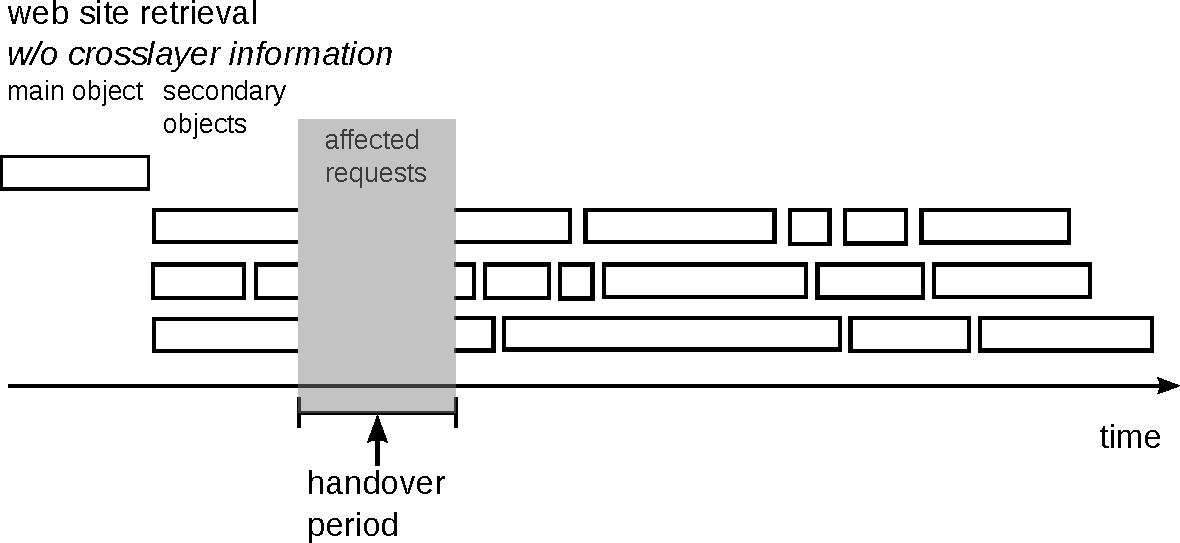
\includegraphics[width=\textwidth]{images/http-reorder-no-cl.pdf}
				\caption{The handover will block currently active object transmissions, page display will be delayed.}
				\label{c5:fig:http-reorder-no-cl}
	        \end{subfigure}%

	        \begin{subfigure}[b]{0.90\textwidth}
				\centering
				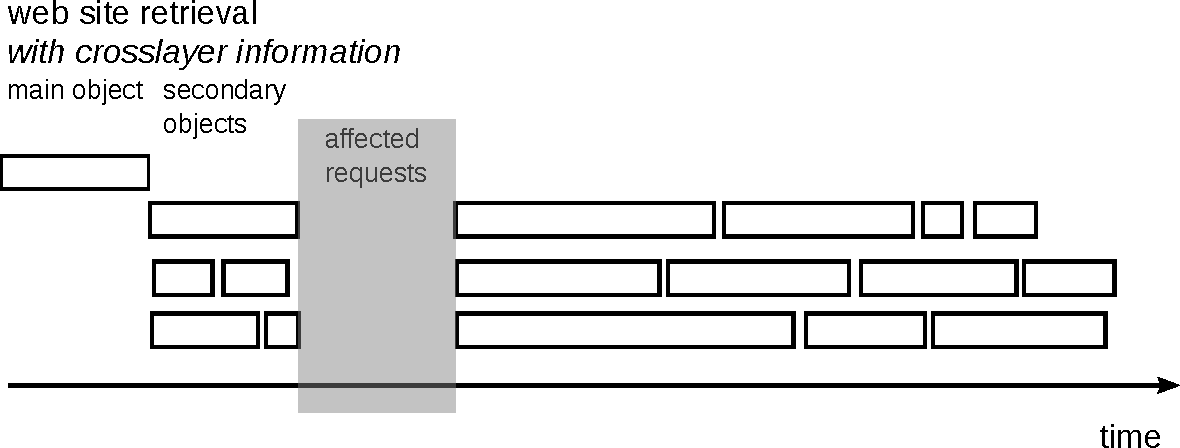
\includegraphics[width=\textwidth]{images/http-reorder-cl.pdf}
				\caption{The browser reorders the objects to be retrieved and avoids any transmissions during the indicated handover period.}
				\label{c5:fig:http-reorder-cl}
			   \end{subfigure}%
	 \caption{Mock-up of \gls{HTTP} reordering with handover awareness.}
	\label{c5:fig:http-reorder}
	\end{figure}

	\item Enable applications to adapt themselves to the conditions currently experienced by the networking stack and its sensors. For example, a Web browser could reorder its Website object requests to avoid sending any requests during handover periods and experience additional delay as seen in Figure~\ref{c5:fig:http-reorder}.

	\item A cross-layer enabled device can also offer a wide range of policy choices to its applications or even directly to the user. An example rule could be: ``Do not handover to a stationary WiFi from 3G when moving faster than 50km/h, only to in-vehicle WiFi.'' or ``Avoid any vertical handover, which would interrupt my service for a long time, while this VoIP call is running.''

\end{itemize}

\subsubsection{Technical Implementation}

The Implementation:
\begin{itemize}
	\item Userspace daemon that collects information from kernelspace protocol implementations and sensors and provides them to all applications.
	\item shared bus control/information system, instead of explicit comm; signaling only to interested parties
	\item provide common interface also to all available sensors and layer 1 and 2 network information and control (similar to Android)
	\item IPC message bus, possibly D-Bus\footnote{\url{http://www.freedesktop.org/wiki/Software/dbus/}} based
	\item Could extend NetworkManager\footnote{\url{https://wiki.gnome.org/Projects/NetworkManager}}, some functionality is already provided there

\end{itemize}

The process:
\begin{itemize}
\item Tell Transport/Application the expected time till handover / time of uninterrupted service
\item Tell Transport/App expected connection parameters (latency, BW, ...)
\item Application selects \gls{DASH} stream appropriate to parameters
\item Application reorders \gls{HTTP} GETs so that large GETs are not interrupted
\item Application stops transfers when handover is about to occur
\item Layer 1/2 gives a list of possible handovers to Application
\item Application selects (better: suggests) handover which fits best and reorders accordingly
\end{itemize}


\subsubsection{Example Benefits}

Put into relation:

\begin{itemize}
	\item frequency of handovers / distance/density of radio towers vs scenario traveling speed
	\item bit-length of streaming segments, typical transmission speed
	\item typical video length and number of segments
	\item derive number of interruptions in segments due to handovers
	\item estimate typical handover/mobility duration and service interruption time per event
	\item sum it up and compare to crosslayer information or even application layer handover decision

\end{itemize}


\subsubsection{Planned Work and Methodology}

\begin{itemize}
	\item investigate how much information is exposed and what can already be done
	\item Analysis of data traces and realistic simulations in order to capture in detail the unwanted phenomena
	\item Verify the suitability of the State-of-the-Art algorithms and protocols which address this problem
\end{itemize}






%%%%%%%%%%%%%%%
%% unused

%Characteristics of UDP packet loss: Effect of tcp traffic \cite{sawashima97characteristics}


%%%%%%%%%%%%%%%%%%%%%%%%%%%%%%%%%%%%%%%%%%%%%%%%%%%%%%%%%%%%%%%%%%%%%%%%%%%%%%%%
%!TEX root = ../../dissertation.tex
%%%%%%%%%%%%%%%%%%%%%%%%%%%%%%%%%%%%%%%%%%%%%%%%%%%%%%%%%%%%%%%%%%%%%%%%%%%%%%%%
\section{Cross-Layer Information Exchange}
\label{c5:sec:crosslayerhinting}

The Internet has its historic roots deep in wired networks with a slim and well-defined network stack represented by the \gls{ISO}/\gls{OSI} or \gls{TCP}/gls{IP} model. These layers are isolated against each other. Only predefined information exchange points, or \gls{osiSAP}, at the layer borders allow for vertical communication. A typical wired \gls{TCP}/\gls{IP} Internet environment rests atop of either an Ethernet or other access technologies, e.g., \acrshort{DSL}, \acrshort{DOCSIS} or \acrshort{PON}, at the physical and link layers.

Application layer protocols often implicitly rely on the presence and characteristics of specific lower layer protocols. Though, through the layer isolation no application can precisely know or even control the current state of the lower layers. Nonetheless, they usually make assumptions on the composition and behavior of the lower layers and plan their work accordingly. 

But the access technology diversity has strongly increased through the advent of wireless technologies, and past fixed access behavioral patterns may not be applicable any more today. The protocols used for the radio transmissions behave very differently when compared to plain Ethernet and higher layers may make false assumptions. Examples for this were given in the in the discussion of the stack's influences in Section~\ref{c5:sec:stack-influences}.

It would be very desirable for transport and application layer mechanisms to be able to better understand these layers and cope with these effects. The term \textit{cross-layer interactions} or \textit{cross layer information exchange} subsumes these approaches. Specific information from one layer is made available to other interested neighboring or more distant layers. Using cross-layer techniques many of the previously introduced negative layer influences can be diminished or neutralized altogether.

The next sections describe related mechanisms in the literature, classifications and then proceed to describe a new cross-layer approach that facilitates cross-layer information to the benefit of mobile streaming. The cross-layer work presented here is rather meant as an initial proposal to be integrated into future streaming players and their playback and transmission strategies.


%%%%%%%%%%%%%%%%%%%%%%%%%%%%%%%%%%%%%%%%%%%%%%%%%%%%%%%%%%%%%%%%%%%%%%%%%%%%%%%%
\subsection{Related Cross-Layer Approaches and Classifications}

The idea of exchanging information between layers is not a particularly new one. Some specific ideas have been implemented a long time ago. The authors of \cite{Raisinghani2004720} list a number of scenarios in which cross-layer information could be used and also talk about the type of information to be shared between layers. One of the oldest and most well known cross-layer approaches is probably \gls{ECN}~\cite{rfc3168}. Here, the \gls{IP} layer of intermediate hops can signal the end nodes' \gls{TCP} layer that congestion is occurring and \gls{TCP} does not need to wait for implicit congestion signals, e.g., duplicate acknowledgments or timeouts. However, \gls{ECN} is disabled in almost every implementation as it lead to numerous problems and triggered bugs\footnote{\url{http://lkml.iu.edu//hypermail/linux/kernel/0009.1/0329.html}}. This is a risk that many cross-layer attempts may face.

A significant amount of publications is dealing with cross-layer information in wireless and mobile protocol stacks. A number of architectures have been proposed, e.g., \cite{raisinghani2004eclair, 1580937}, \cite{wang2003multi}, \cite{1200522}, and \cite{krishna2007cross}, but no actual solution seems to have been implemented in any of these.

While cross-layer typically implies a solely \textbf{vertical} --- between network layers --- exchange flow there can also be \textbf{horizontal} --- between network nodes --- components present. \gls{DLEP}~\cite{ietf2013dlepdraft} is such an example of a \textbf{diagonal} flow, providing information of a lower layer of one entity to a higher layer at another node. The \gls{DLEP}~\cite{ietf2013dlepdraft,6379143} protocol provides information available only to the (external) wireless modem or other interfaces to the routing entity of a node upon which it can act. Link characteristics such as bandwidth, latency, connection status, or information regarding neighbors can be requested.

Though, horizontal information flow in cross-layer approaches is more than often an indication of \textbf{centralization} (also called \textbf{network-assisted} or \textbf{managed}) as apposed to purely vertical \textbf{distributed} approaches. Concerning this network-assisted cross-layer exchange there are a number of approaches that aim to integrate layer cooperation into the design of new mobile network infrastructures, including \cite{zarai2010seamless} and \cite{Piamrat20111066}. Generally, information is retrieved from the clients and collected at a central manager to be used in any policy decision like mobility and radio resource management.

Going back to purely distributed approaches, in \cite{hummel2010mobilitaet} the concept of mobility awareness is discussed. The goal is to predict motion and mobility based on available information and adapt the individual network layers to react accordingly. One of the easiest to implement uses of cross-layer information is the selection of the active network interface. Current mobile devices have a wide range of network interfaces available, all with specific characteristics. The management architecture proposed in  \cite{Bonnin:2009:AMM:1503496.1503498} switches the currently used interface based on pre-configured profiles. Information from multiple layers is used to support the decision-making process.

To optimize unreliable video streaming in a WiFi network, the authors of \cite{1580941} create a control loop between the video encoder and the 802.11 \gls{MAC} layer to conduct WiFi rate control fitted to the output of the encoder. This is an example of a tight cross-layer control loop for one particular application. The link layer rate control will very likely have adverse affects on other applications using this node.

The notion of cross-layer can also be applied to non-traditional network stacks. For example, the authors of \cite{4656786} present a cross-layer model for satellite communication stacks. They additionally distinguish between two general flavors of cross-layer architectures, one with \textbf{direct} and the other with \textbf{indirect} communication. Direct exchange implements new vertical interfaces in the layers and exchanges information directly between them. The indirect alternative uses an external information broker that handles all communication in parallel to the existing layers. Similar cross-layer information can be offered to peer-to-peer overlay networks, as was for example researched in the SmoothIT project\footnote{\url{http://www.smoothit.org}}, where routing and topology information was collected and made available to interested peers~\cite{oechsner2009pushing} in order to keep traffic local and avoid using \acrshort{ISP} interdomain links.


%%%%%%%%%%%%%%%%%%%%%%%%%%%%%%%%%%%%%%%%%%%%%%%%%%%%%%%%%%%%%%%%%%%%%%%%%%%%%%%%
\subsection{Cross-Layer Model and Implications}

With these past approaches and classifications at hand, a cross-layer model suitable for video streaming in mobile networks can now be defined and the information to be exchanged specified.

\begin{figure}[htb]
	\centering
	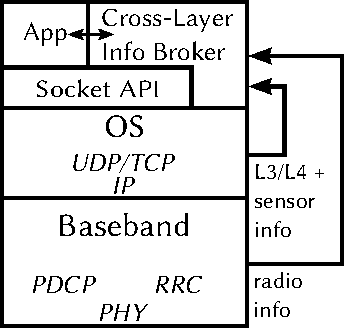
\includegraphics[width=0.3\textwidth]{images/cross-layer-model.pdf}
	\caption{Model and architecture of the proposed cross-layer information exchange.}
\label{c5:fig:crosslayer-model}
\end{figure}

Figure~\ref{c5:fig:crosslayer-model} illustrates the concept with the example of a mobile device. In a fully isolated model, no information would be passed from the baseband to the \gls{os} and the applications. The cross-layer model permits certain information to pass from one layer to another. Here, a software broker is responsible to collect information from several sources and layers and make it available to any interested application in a concise manner. 

This is an indirect cross-layer approach bypassing the intermediate layers completely and leaving them mostly unmodified. Also, information is always collected and used on the same device, making it purely vertical and distributed. Sharing this kind of information between different hosts would be accompanied by certain privacy and security implications. Most of the data is very sensitive and also be used with malicious intent if it is being leaked by a cross-layer broker.

This architecture is intended to pass data from the physical and link layer directly up to the application. Especially information specific to \gls{3G} mobile networks could be potentially interesting and used in benefit for applications and the user experience.This could include:

\begin{itemize}
	\item Information on the occurrence of a horizontal handover between cells.

	\item Information on neighboring cells and predictions when a handover is most probable to occur.

	\item Information on the prediction of the occurrence of a vertical handover and thereby changes in the active network stack, e.g., to the WiFi layers.

	\item Information on the current signal strength, bit error rate, and throughput.

	\item Detailed mobility information, including current location and travel speed in relation to base station positioning and availability.
\end{itemize}

Today, most of this information is only available inside the link layer or even just known to the mobile network's control plane. The impact of a lack of this knowledge can be significant for applications. For example, traffic scheduled during a handover period can be subject to especially high latency and loss due to the lengthy control plane interactions and traffic rerouting processes in a mobile network. If a cross-layer exchange would be provided and the application is made aware when an handover is supposed to occur, traffic could be scheduled around the event. 

Generally speaking, the goal of the cross-layer approach would be to find meaningful reactions for every type of state the lower layers report through the broker. The pool of recipients is also not necessarily limited solely to the application layer. Especially the transport layer could be interested into explicit connectivity information and be modified to react accordingly. In addition to information flow, a path for control flow could also be envisioned. Herein, applications could directly influence the decision making and policies of the lower layers and adapt them to their personal needs.

All in all, the cross-layer data needs as well as the recipient's reactions need to be well defined and thoroughly tested to avoid any conflicts and layer separation issues. The impact of a simple unidirectional information flow on the layering mechanisms is suggested to be rather low. Only explicit and specific information is revealed keeping most of the isolation intact. However, a bidirectional control flow could soften up the isolation and have adverse side-effects through conflicting interests of participating applications.

Either way, when implementing any kind of cross-layer exchange, one always has to keep a close look on the resulting consequences. One side effect can be the creation of an unintentional feedback loop between the control mechanisms of protocols of different layers. Moreover, breaches in the isolation could leak network state that could be exploited by malicious parties in any number of unforeseeable ways. Therefore, handling these plays an important role in cross-layer research. In \cite{1404568} the authors present and discuss some of these issues.


%%%%%%%%%%%%%%%%%%%%%%%%%%%%%%%%%%%%%%%%%%%%%%%%%%%%%%%%%%%%%%%%%%%%%%%%%%%%%%%%
\subsection{Utilizing Cross-Layer Information for Adaptive Reliable Streaming in Mobile Networks}

Looking at the model it can be an obvious fit for adaptive reliable streaming. As introduced in Section~\ref{c3:sec:background}, adaptive streaming usually facilitates a segment-based pull approach on top of \gls{HTTP}. A local video buffer is maintained and attempted to be kept between predefined thresholds. The goal is to never run out of buffered video while still providing the best possible quality, which could be difficult to achieve in a highly variable mobile network.

Cross-layer information can be fed into the adaptivity model of the streaming player to better decide the exact schedule and quality level of segment transmissions. Adaptive reliable streaming can be especially suited to receive cross-layer data for several reasons: First, all requests are client-initiated, so available information can be immediately taken into account and does not need to be transfered elsewhere. Second, adaptive streaming consists of small and independent video segments, which allows to quickly react on upcoming events.

\begin{figure}[htb]
	\centering
	\begin{subfigure}[b]{0.80\textwidth}
		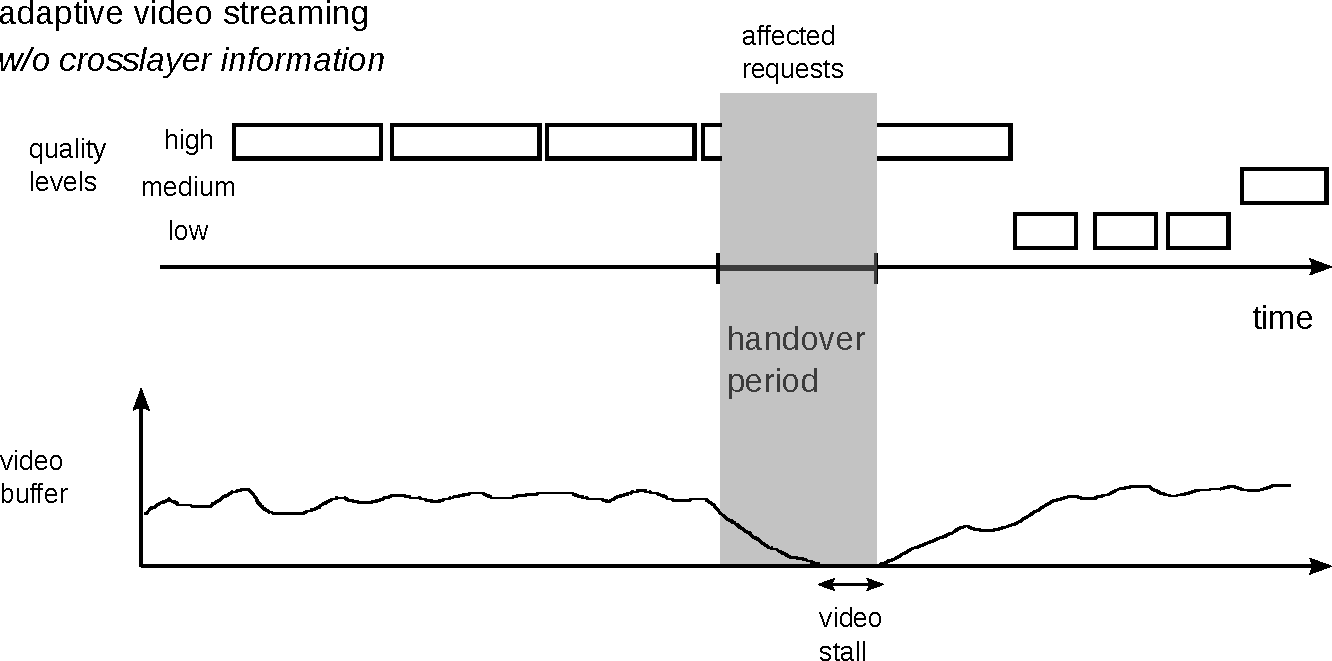
\includegraphics[width=\textwidth]{images/adaptive-streaming-no-cl.pdf}
		\caption{Stalling occurs without handover hinting.}
		\label{c5:fig:streaming-hinting-no-cl}
	\end{subfigure}%

	\begin{subfigure}[b]{0.80\textwidth}
		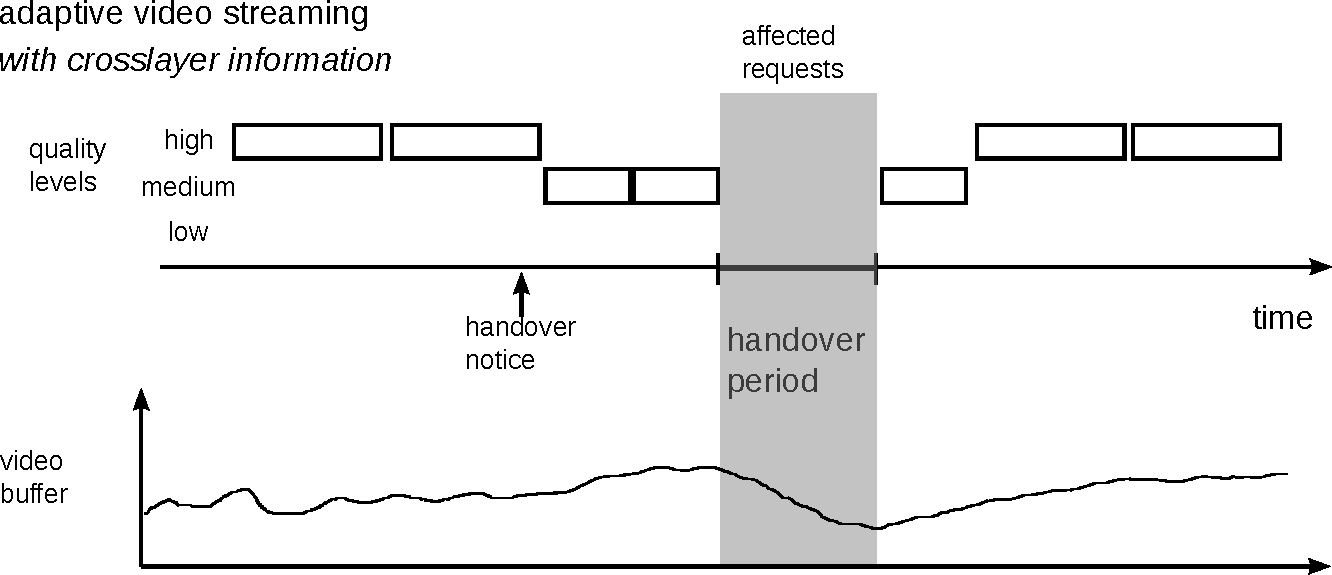
\includegraphics[width=\textwidth]{images/adaptive-streaming-cl.pdf}
		\caption{Stalling can be prevented by hinting and proactively filling the playback buffer.}
		\label{c5:fig:streaming-hinting-cl}
	\end{subfigure}%
	\caption{Adaptive video streaming scenario with and without handover prediction and cross-layer hinting.}
\label{c5:fig:streaming-hinting}
\end{figure}

One of the easiest events to improve upon is the timely knowledge (or prediction) of upcoming handover procedures, horizontal as well as vertical handovers. Consider the scenario given in Figure~\ref{c5:fig:streaming-hinting-no-cl}. The streaming player consistently retrieves video segments at the highest quality, maintaining a moderate buffer size but oblivious to the upcoming handover. This handover interrupts any transmission for a certain time, during which the buffer is fully drained and the video playback begins to stall. Only after this phase ended, the remaining portion of the segment can be received. But the buffered amount is now still below the safety margin and the player is forced to request several segments in the lowest quality to quickly refill the buffer. Only after that, the player's state normalizes and normal quality playback is restored. In summary, one unexpected service interruption causes one complete stall and a long period of reduced quality in this exemplary scenario. This effect can also be easily observed in the mobile reliable streaming simulation scenario described in Section~\ref{c6:sec:mobilitystreamingsim}.

Figure~\ref{c5:fig:streaming-hinting-cl} shows the same scenario but with cross-layer hinting present. As soon as the notice of a predicted upcoming handover is received, the streaming player can react and switch to segments with medium quality to increase the buffer size before the event. After the handover has completed one more medium segment is transmitted to get the buffer level back to normal before returning to full quality. Both the video stalling period and the drop to the lowest quality could be avoided here. The general goal in the streaming process is to both stop the buffer from ever completely emptying and also maintaining the highest possible video quality. To achieve this, early knowledge of future network conditions is highly desirable for the streaming controller to correctly adjust the segment retrieval rate and quality.

The end-to-end concept can be applied to cross-layer architectures as well. While cross-layer information can still be made available to intermediate layers, the achievable effects might either not be as large as in the highest layer or more complicated to attain. For example, it requires much more effort to correctly adjust \gls{TCP} retransmissions and congestion control to accommodate the cross-layer broker without side-effects to other applications. Nonetheless, benefits can still be attained at the transport layer to some degree if the adjustments are being kept application-neutral. This can be especially helpful for applications that have not yet been adapted to handle cross-layer information.


%%%%%%%%%%%%%%%%%%%%%%%%%%%%%%%%%%%%%%%%%%%%%%%%%%%%%%%%%%%%%%%%%%%%%%%%%%%%%%%%
\subsection{Benefits for Other Applications}

Besides this work's central motifs of reliable streaming, other applications could benefit as well. First, cross-layer information could be utilized to directly improve the user interface and experience. Any information of upcoming service interruptions or other adverse conditions are simply displayed to the user. This is specifically helpful for interactive communication --- as in video calls or \gls{VoIP}. An unsuspecting user might be more startled at a sudden loss of reception than the one that was informed beforehand. The communication partner can additionally also be informed. While user hinting and notifications does generally not actually improve the actual \gls{QoS} of the application it can still positively improve the perceived quality or \gls{QoE}. But detailed user studies would need to verify this further.

Generally, any application that can locally exert control over its traffic and does not have to rely on server-side control will benefit the most. Also, the traffic should be ideally composed of smaller objects available in multiple versions and free to be reordered. A good candidate would be Web browsers with their stateless \gls{HTTP} requests of a Web site, which is comprised of many small objects that can be, to a certain degree, requested in any order. Those objects could be requested in such an order to better accommodate network events announced by the lower layers. On the other hand, \gls{rtp}-style streaming traffic might not be able to beneficially utilize cross-layer information as just a stream of continuous data is pushed to onto the client.

Directly involving the user itself are a further category of cross-layer interactions that are only available if there is a downward control flow through the broker to the radio layer protocols. This would require the additional presence of a user-space policy manager. The manager would offer the user a series of preferences and a configuration interface for a rule-based cross-layer control engine. With this the user could create complex compound policies such as: ``Do not handover to a stationary WiFi from \gls{3G} when moving faster than \SI{50}{\kilo\meter\per\hour}, switch only to in-vehicle WiFi if available.'' or ``Avoid any vertical handover, which would interrupt my service for a long time, while a \acrshort{VoIP} call is running.''


%%%%%%%%%%%%%%%%%%%%%%%%%%%%%%%%%%%%%%%%%%%%%%%%%%%%%%%%%%%%%%%%%%%%%%%%%%%%%%%%
\subsection{Implementation Outlook and Approaches}

As the model displayed, the target applications should not be directly (or indirectly through the inclusion of a third-party software library) responsible to retrieve cross-layer information. Instead, the broker was suggested as the means to implement cross-layer exchange in an actual software environment. This daemon --- located in the user space --- collects information from the lower layer network protocols which usually reside entirely in kernel space. The kernel typically exposes only some data publicly with a stable \gls{API} and \gls{ABI}. Other data can often be derived from internal data structures which usually change with every version. The task of adapting to this changes and collecting concise data is handled by the daemon. Only the actual reactions to these information points must be implemented in the application itself.

The daemon provides all information through a pre-defined user space interface to interested parties. This includes the raw data itself, e.g., current latency or bandwidth information, as well as derived and predicted data points. Examples for the latter are the discussed early handover warning or mobility predictions. To further improve predicted values the daemon also integrates data from other device sensors outside the classical network stack, amongst others location and movement data and as well as system and battery state.

To further decouple the applications from the broker, the information should be provided through a shared \gls{IPC} bus. Current candidates for the reference implementation are Android, using the provided Intent\footnote{\url{https://developer.android.com/reference/android/content/Intent.html}} \gls{IPC} mechanism, as well as Linux distributions using D-Bus\footnote{\url{http://www.freedesktop.org/wiki/Software/dbus/}}. An even higher level implementation might be possible for the latter case, as the D-Bus-based NetworkManager\footnote{\url{https://wiki.gnome.org/Projects/NetworkManager}} framework already provides some of the network-related functionality. For example, it would be rather simple to implement switching the active network interface on the basis of cross-layer data with NetworkManager.

Through these decoupling efforts the broker's implementation and binary package can be completely swapped with another and all applications still work, as long as the bus interface stays the same. Therefore, the user and her chosen applications is not bound to a specific cross-layer broker provider with predictions conducted by certain algorithms. Rather, she can easily supplant the existing provider with a better one. The planned broker is therefore only meant as a reference implementation. Additionally multiple brokers could even be simultaneously active as long as as long as their provided data does not intersect.

The viability of cross-layer information can be evaluated in several ways. A pure network-level simulation can give initial hints on performance gains and issues. But only the evaluation of data traces and packet level captures of an actual reference implementation might give good insights into the implications of diminishing the network stack's layer encapsulation properties. A further comparative statistical analysis of several different approaches to cross-layer data predictions algorithms as well as the specific application's reactions could also prove to be of significant interest. Both the testbed and \gls{LTE} simulation approaches developed in Section~\ref{c6:sec:mobilestreamingtestbed} can help in validating this cross-layer approach.



% influence of signaling plane and core network elements - scaling
%This can apply to, e.g., reliability, frame sizing and fragmenting, and latency amounting to undesired effects on higher-layer traffic. 

 %Modem Link Properties Advertisement Protocol\footnote{\url{https://tools.ietf.org/html/draft-ivancic-mobopts-modemlpa-01}}

%LCP Link Control Protocol, PPP extension RFCs \cite{rfc1570,rfc1661}
%LISP and other mobility approaches \cite{rfc6830}

% Conceptually similar to cross-layer interactions is the family of dynamic radio resource management techniques. These control many properties concerning radio resources. 
% Radio Resource Management RRM
% 		\begin{itemize}
% 			\item resource monitoring, decision making, decision enforcement
% 			\item choose available wireless interfaces  best suited for a specific task
% 			\item rudimentary implementations in mobile OSs
% 		\end{itemize}
%	IEEE 802.21 cooperative handovers, but with required network support
%  Cross-layer design for wireless networks \cite{1235598} keine wirkliche aussage zu cross-layer

% User-centric mobility management for multimedia content access \cite{bolla2011usercentric} (not really cross-layer, uses something similar to LISP: an additional identifier shim and session migration for rtsp/sip) oddly mixed with user questionnaires

% Socketless \gls{TCP} --- an end to end handover solution \cite{1635680} % mobility scheme, not actually cross-layer information

%A ubiquitous mobile communication architecture for next-generation heterogeneous wireless systems \cite{1452832} (supposed to propose a function that determines the best handover initiation time in order to avoid early or late initiations)



	% - Research objectives
	% 	- Bidirectional vertical information and control flow on the performance of the individual layers
	% 		- Definition of generic interfaces
	% 		- Definition of a protocol (including information types, etc.)
	% 	- Definition of meaningful actions/reactions on the individual layers (e.g. adaptation of real-time communication data sources or changes in resource allocation)


%Using current location data and movement patterns/predictions to improve cell selections and initiate horizontal and vertical handovers to a time suitable for the device and running applications.


% For example, a Web browser could reorder its Website object requests to avoid sending any requests during handover periods and experience additional delay as seen in Figure~\ref{c5:fig:http-reorder}.
% 	\begin{figure}[htb]
% 	        \centering
% 	        \begin{subfigure}[b]{0.90\textwidth}
% 	            \centering
% 				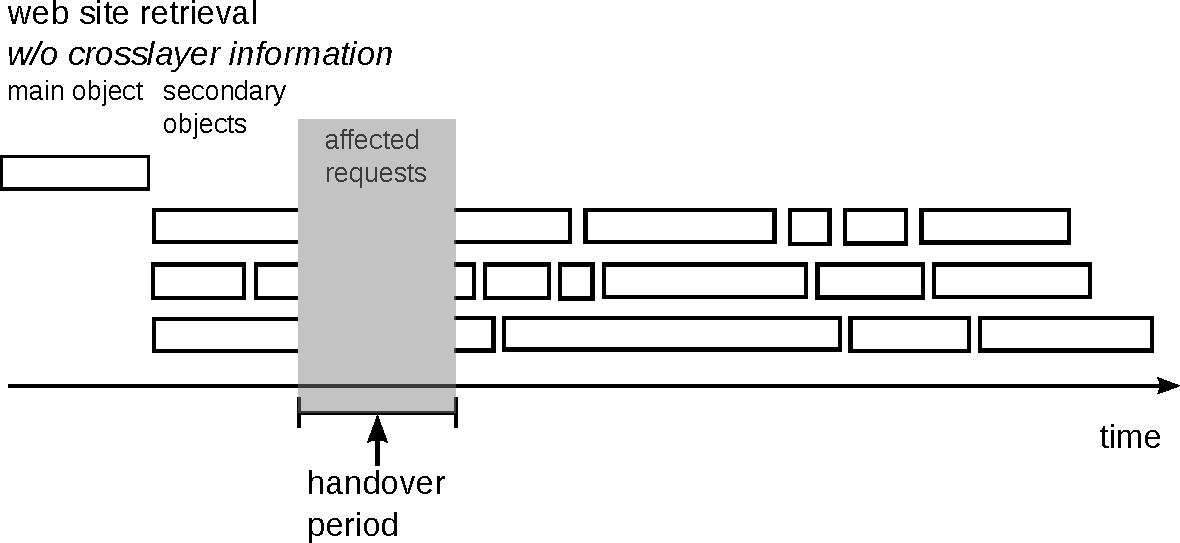
\includegraphics[width=\textwidth]{images/http-reorder-no-cl.pdf}
% 				\caption{The handover will block currently active object transmissions, page display will be delayed.}
% 				\label{c5:fig:http-reorder-no-cl}
% 	        \end{subfigure}%

% 	        \begin{subfigure}[b]{0.90\textwidth}
% 				\centering
% 				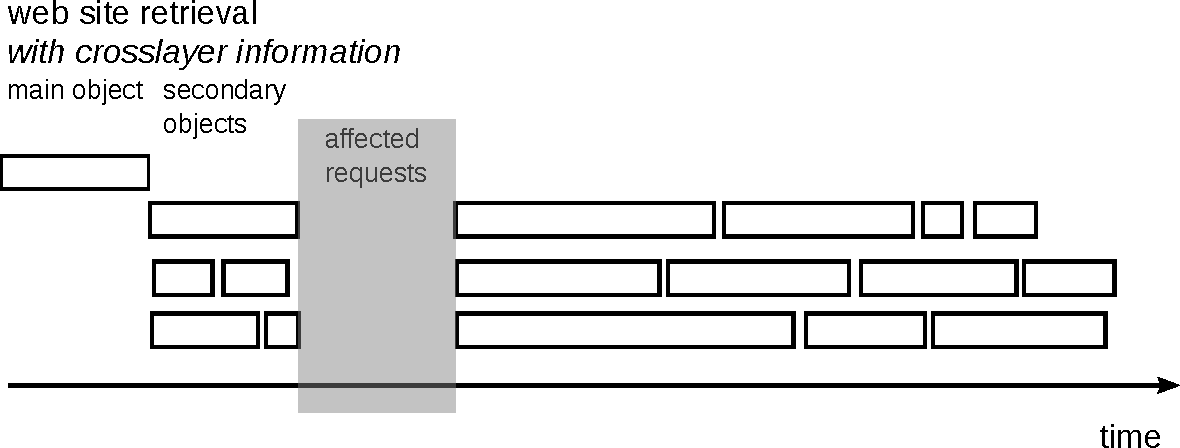
\includegraphics[width=\textwidth]{images/http-reorder-cl.pdf}
% 				\caption{The browser reorders the objects to be retrieved and avoids any transmissions during the indicated handover period.}
% 				\label{c5:fig:http-reorder-cl}
% 			   \end{subfigure}%
% 	 \caption{Mock-up of \gls{HTTP} reordering with handover awareness.}
% 	\label{c5:fig:http-reorder}
% 	\end{figure}



%Put into relation:
% \begin{itemize}
% 	\item frequency of handovers / distance/density of radio towers vs scenario traveling speed
% 	\item bit-length of streaming segments, typical transmission speed
% 	\item typical video length and number of segments
% 	\item derive number of interruptions in segments due to handovers
% 	\item estimate typical handover/mobility duration and service interruption time per event
% 	\item sum it up and compare to crosslayer information or even application layer handover decision
% \end{itemize}


%%%%%%%%%%%%%%%%%%%%%%%%%%%%%%%%%%%%%%%%%%%%%%%%%%%%%%%%%%%%%%%%%%%%%%%%%%%%%%%%
\section{Mobile Streaming Summary}

To summarize, application layer protocols are sensitive to circumstances of the lower protocol layers. Reliable streaming is no exception to this rule. Due to the time constraints present in media streaming it might even be more sensitive to outside influences than some other protocol with more relaxed timing constraints. Those protocol layer influences are aplenty, especially in mobile networks, and are most often unintended side effects of some protocol feature or behavior.

But this Chapter showed, that the mobile and Internet protocol stack is still very much in ongoing development and many of these side effects are known and being worked on. This happens either through the replacement of old protocols with entirely new versions, that attempt avoid these influences, or changes to existing protocols, as can be most prominently seen in the steady changes to \gls{TCP}. However, as it might not be enough to improve the individual layers, a concept for cross-layer cooperation between protocols on different layers is also highly desirable. The framework provided here should serve as a blueprint for future reliable applications to correctly facilitate information from the mobile network, e.g. handover event information.


